\documentclass[table, 12pt]{article}
\usepackage[T1]{fontenc}
\usepackage[utf8]{inputenc}
\usepackage[english]{babel}
\usepackage{graphicx}
\usepackage{titlesec}
\usepackage{hyperref}
\usepackage[usenames,dvipsnames]{xcolor}
\usepackage{float}
\usepackage[export]{adjustbox}
\usepackage{longtable}

\hyphenation{Te-lan-ga-na}
\hyphenation{an-a-lys-ing}
\hyphenation{a-gron-o-mists}
\hyphenation{a-gron-o-mist}
\titleformat{\paragraph}
{\normalfont\normalsize\bfseries}{\theparagraph}{1em}{}
\titlespacing*{\paragraph}
{0pt}{3.25ex plus 1ex minus .2ex}{1.5ex plus .2ex}


\begin{document}
\begin{titlepage}
    \centering
    {\scshape\large AY 2021/2022 \par}
    \vfill
    
\includegraphics[width=100pt]{assets/logo-polimi-new}\par\vspace{1cm}
    {\scshape\LARGE Politecnico di Milano \par}
    \vspace{1.5cm}
    {\huge\bfseries DD\@: Design Document \par}
    \vspace{2cm}
    {\Large {Ottavia Belotti\quad Alessio Braccini\quad Riccardo Izzo}\par}
    \vfill
    {\large Professor\par
        Elisabetta \textsc{Di Nitto}}
    \vfill
    {\large \textbf{Version 1.0}\\ \today \par}
\end{titlepage}

\hypersetup{%
    pdfborder = {0 0 0}
}

\thispagestyle{plain}
\pagenumbering{gobble}
\mbox{}
\newpage
\pagenumbering{roman}
\tableofcontents
\newpage
\pagenumbering{arabic}

\section{Introduction}


\subsection{Purpose}
The purpose of this document is to provide a full technical description of the system described in the RASD document.
In this design document we discuss about both hardware and software architectures in terms of interaction among the components that represent the system.
Moreover there are mentions about the implementation, testing and integration process.
This document will include technical language so is primarily addressed to programmers but stakeholders are also invited to read it in order to understand the characteristics of the project.

\subsection{Scope}
The scope of this design document is to define the behavior of the system in both general and critical cases, and to design the architecture of the system by describing
logical allocation of the components and the interaction between them.
This document also extends in part to the implementation and testing plan, where one possible course of action is explained, user interface design of user applications and requirements traceability relating to the RASD.
\subsection{Definitions, acronyms, abbreviations}
\subsubsection*{Acronyms}
\begin{itemize}
    \item \textbf{DREAM}: \emph{Data-driven predictive farming}
    \item \textbf{RASD}: Requirement Analysis and Specification Document
    \item \textbf{DD}: Design Document
    \item \textbf{API}: Application Programming Interface
    \item \textbf{DBMS}: Database Management System
    \item \textbf{UML}: Unified Modeling Language
    \item \textbf{GPS}: Global Positioning System
    \item \textbf{IT}: Information Technology
    \item \textbf{GUI}: Graphic User Interface
\end{itemize}
\subsection{Revision history}

\subsection{Reference documents}
\begin{itemize}
    \item Specification document: "Assignment RDD AY 2021-2022"
    \item Requirements Analysis Specification Document (RASD)
    \item UML documentation: https://www.uml-diagrams.org/
    \item ArchiMate documentation: https://pubs.opengroup.org/architecture/archimate3-doc/
    \item Slides of the lectures
\end{itemize}
\subsection{Document structure}
\begin{itemize}
    \item \textbf{Section 1} gives a brief description of the design document, it describes the purpose and the scope of it including all the definitions, acronyms and abbreviations used. 
    \item \textbf{Section 2} delves deeply into the system architecture by providing a detailed description of the components, the interfaces and all the technical choices made for the development of the application.
    It also includes detailed sequence, component and ArchiMate diagrams that describes in depth the system.
    \item \textbf{Section 3} contains a complete description of the user interface, it includes all the client-side mockups with some graphs useful to understand the correct execution flow.
    \item \textbf{Section 4} links the RASD and the DD, it maps the goals and the requirements described in the RASD to the actual functionalities presented in this DD.
    \item \textbf{Section 5} presents a description of the implementation, testing and integration phases of the system components.
\end{itemize}
\section{Architectural Design}


\subsection{Overview}
\begin{center}
    \begin{figure}[H]
        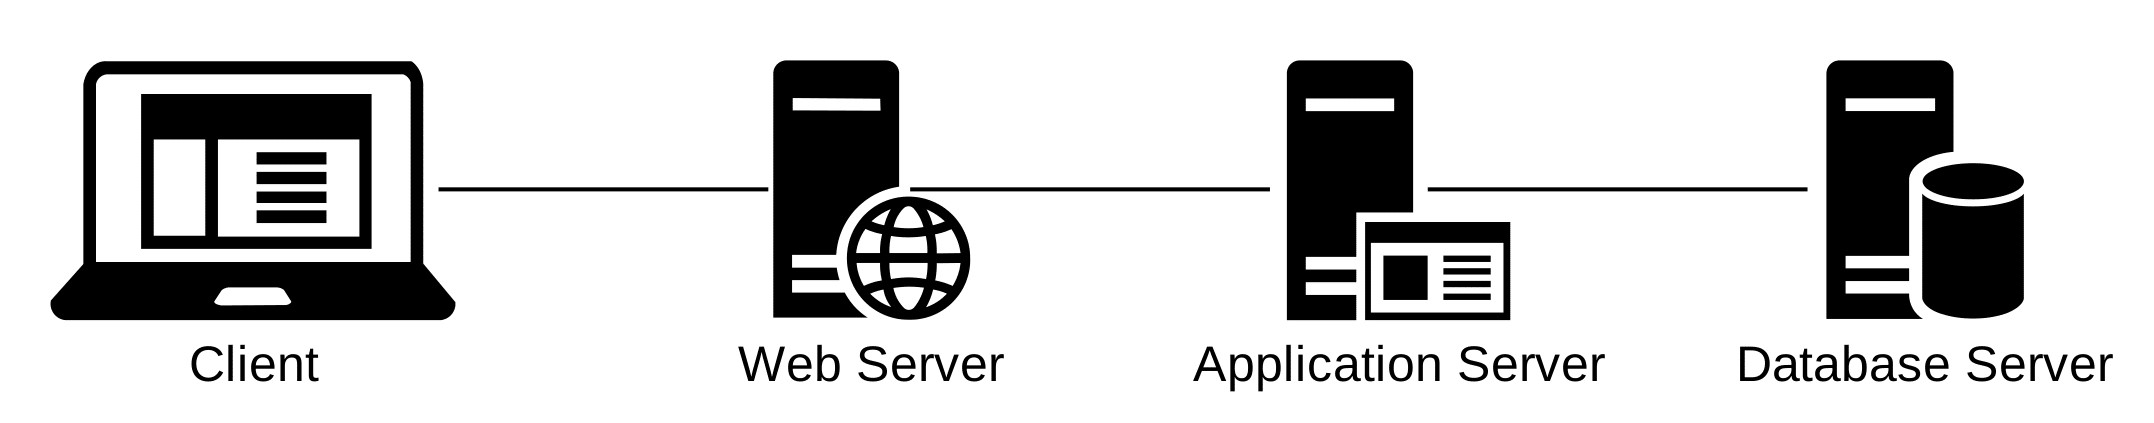
\includegraphics[scale=0.55, center]{assets/4-tier-scheme.jpg}
        \caption{Four-Tier Architecture Scheme}
        \label{fig: four-tier-architecture-scheme}
    \end{figure}
\end{center}

The system is a distributed application that follow the common client-server paradigm.
The architecture of the application is structured in three logic layers:
\begin{itemize}
    \item \textbf{Presentation Layer (P)}: it manages the presentation logic and handles the user actions.
    It is characterized by a GUI (Graphic User Interface) that allow the user to interact with the application in a simple and effective way.
    \item \textbf{Logic or Application Layer (A)}: it manages all the functionalities that has to be provided to the users, it is also responsible of data exchange between the client and the data sources.
    \item \textbf{Data Layer (D)}: it manages the access to data sources, it gets data from the database and move them through the other layers.
    It is essential to guarantee a high level of abstraction from the database in order to provide a model easy to use.
\end{itemize}

\begin{center}
    \begin{figure}[H]
        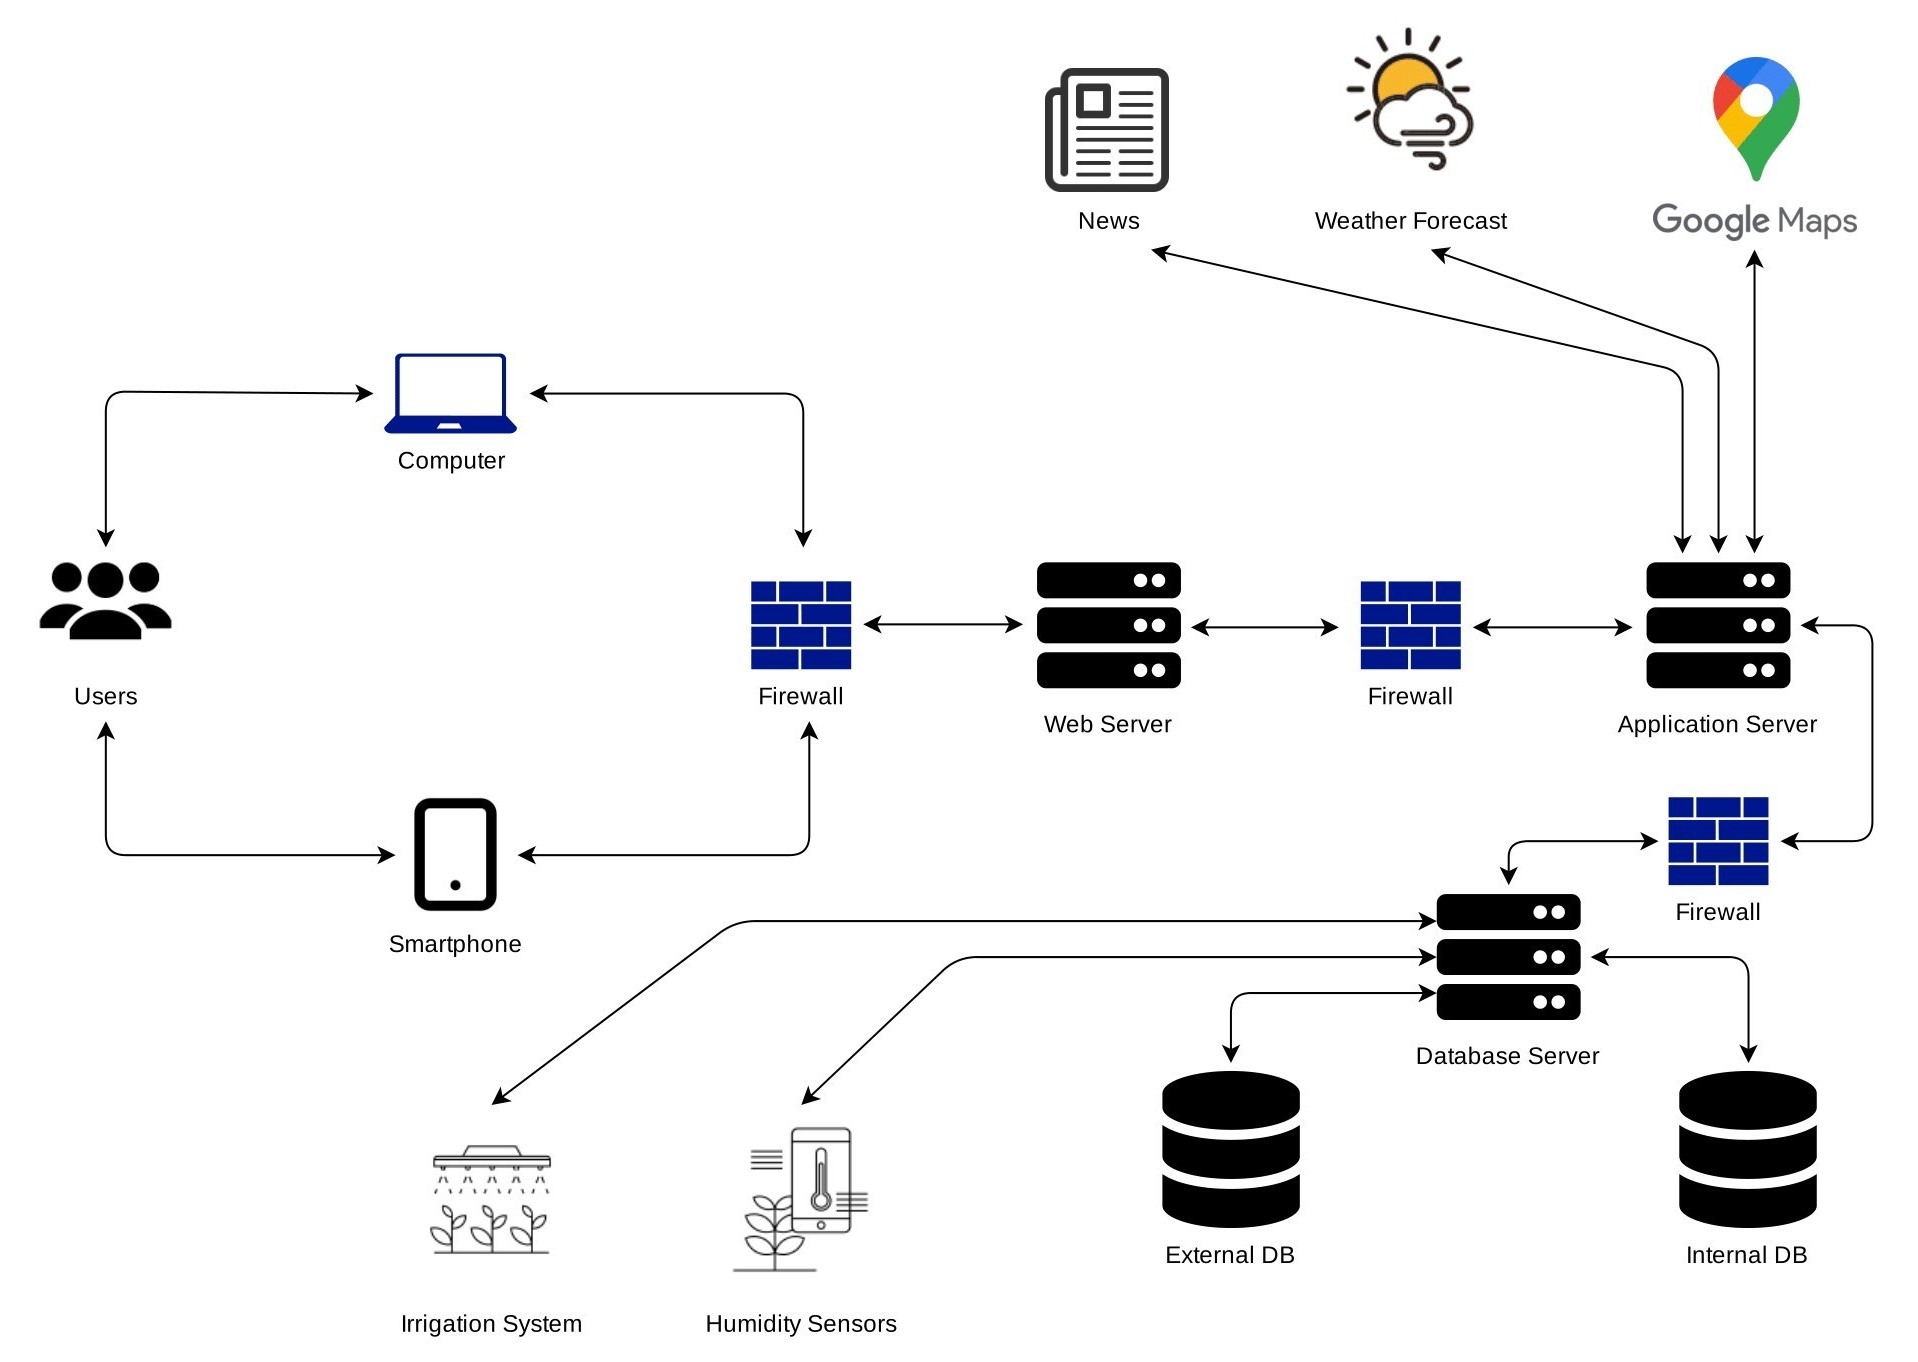
\includegraphics[scale=0.70, center]{assets/4-tier-architecture-scheme.jpg}
        \caption{High Level Architecture}
        \label{fig: high_level_architecture}
    \end{figure}
\end{center}

The system, as shown in \textit{Figure (\ref{fig: four-tier-architecture-scheme})}, is based on a four-tier architecture (Client, Web Server, Application Server and Database Server), this ensures more flexibility and high scalability.
The tiers are separated by firewalls in order to guarantee a higher level of security of the whole system.
A thin client is used to prevent heavy computation load client side, all the heavy operations are executed at the server side.
The client's devices can be a personal computer or a mobile device, both communicate directly with the Web Server through a web browser.
The Application Server communicates with the Database Server and transform data with business logic.
It also manages the news and the weather forecast services.
This allow to retrieve data like the weather directly from it in order to show them to the user.
Finally, to enable the geolocalization, the Application Server uses the API provided by Google Maps.
For what concern the other components, such as the water irrigation system and the humidity sensors, they are connected to the Database Server that exchange data with the Application Server.
The Web Server also manages the data coming from the irrigation system and the humidity sensors.
All the components will be described in depth in the following sections.

\subsection{Component view}
\subsubsection*{General Component View}
\begin{center}
    \begin{figure}[H]
        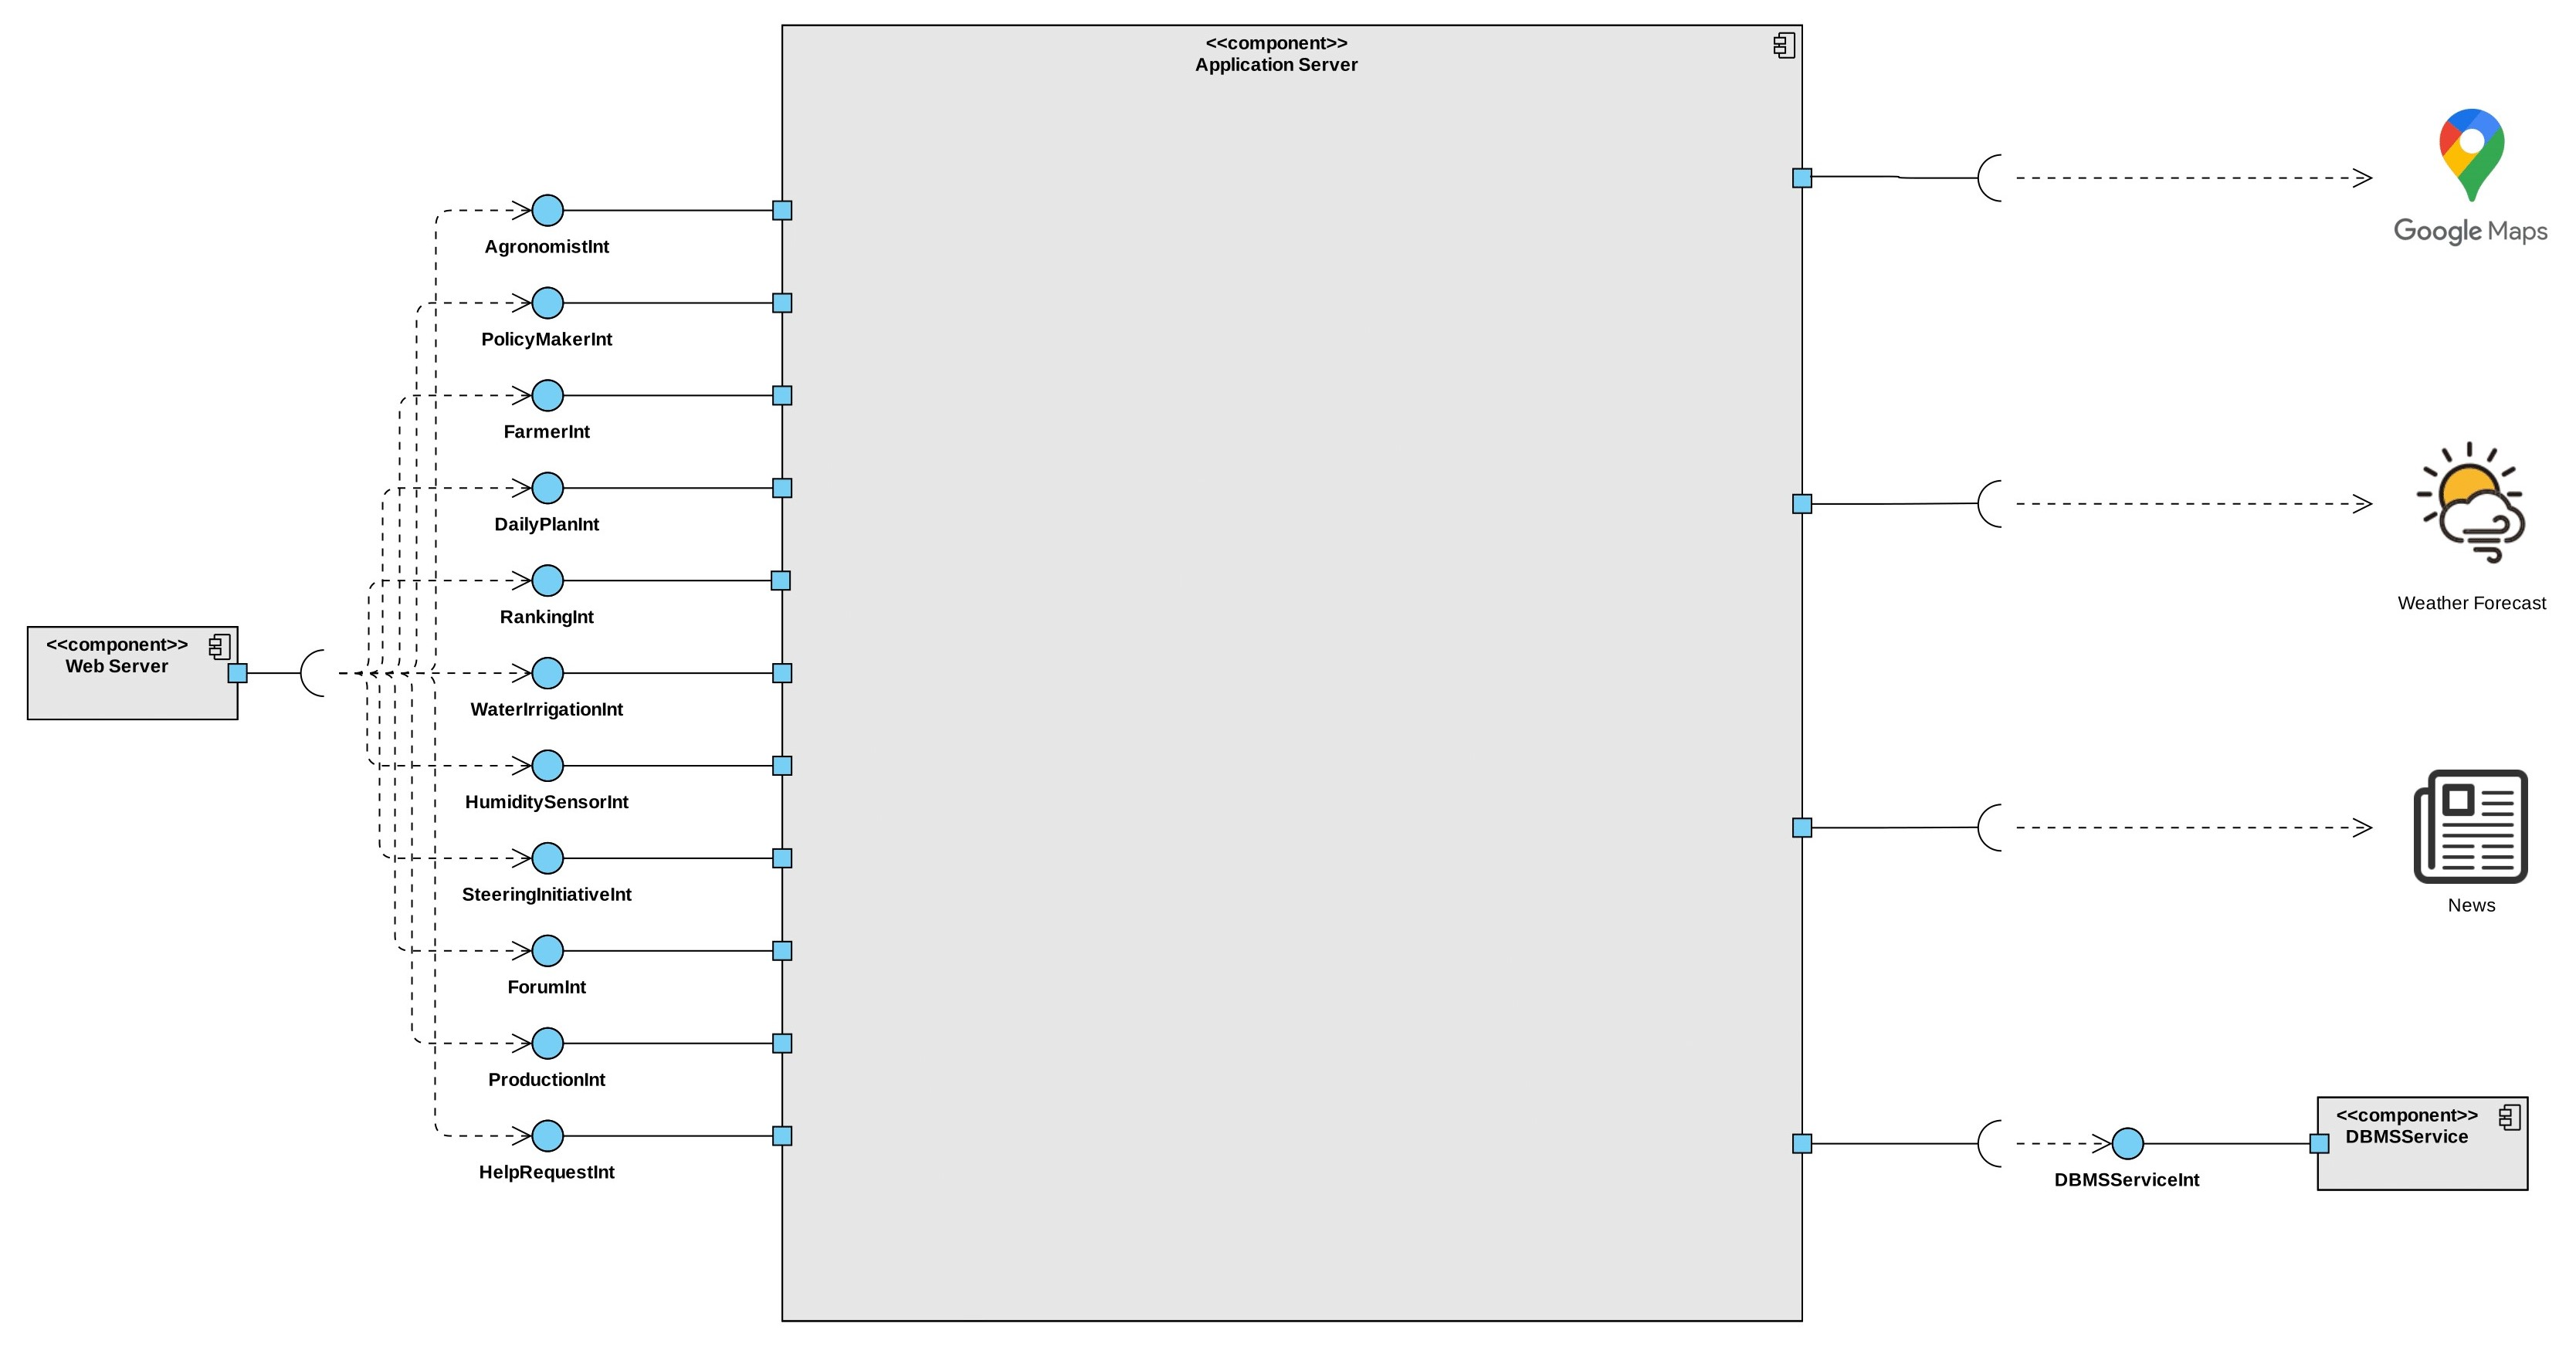
\includegraphics[scale=0.50, center]{assets/general-component-view.jpg}
        \caption{General Component Diagram}
        \label{fig: general_component_view}
    \end{figure}
\end{center}

This image gives an high level representation of the components of the system.
On the left are shown the provided interfaces between the Web Server and the Application Server that in this scheme is represented as a "black box", a complete description of it is provided in the next section.
All the interfaces basically represents the main functionalities requested by the client application.
On the right there are the requested interfaces, one of this is responsible of the geolocalization and is provided by the Google Maps API.
Moreover there are two interfaces that manage the weather forecast and the news services.
Finally, the DBMS interface manages the DBMS service and is responsible of the communication between the Application Server and the Database Server.

\subsubsection*{Application Server Component View}
\begin{center}
    \begin{figure}[H]
        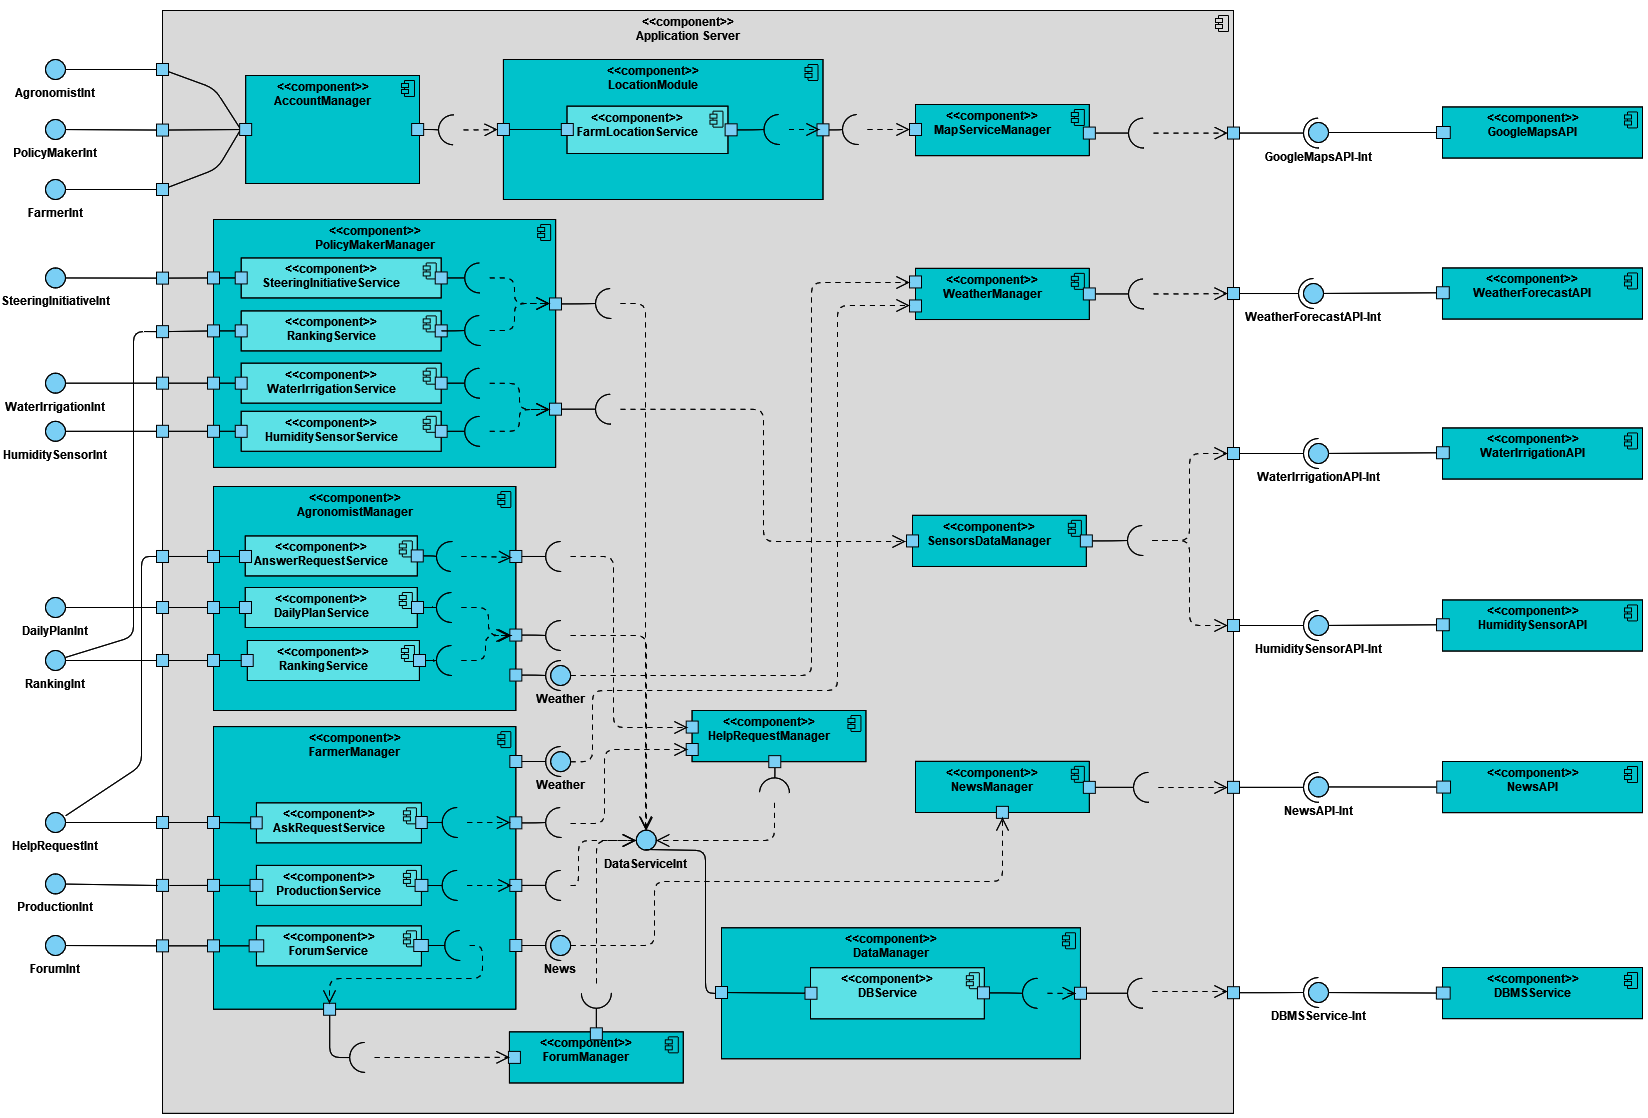
\includegraphics[scale=0.45, center]{assets/application-server-component.png}
        \caption{Application Server Component Diagram}
        \label{fig: application_server_component_view}
    \end{figure}
\end{center}

The following component diagram gives a detailed view of the Application Server, it shows the internal structure and the interaction between the components.
External elements in the diagram are represented in a simplified way.
\begin{itemize}
    \item \textbf{AccountManager}: this component handles all the basic requests made by the client.
    This includes the authentication process that is composed by the log in, the log out and the sign up services. 
    It also includes the edit profile process responsible of the editing of the user account.
    Once a user is logged in, all the specific functionalities are provided by the component that manages this type of user.
    Finally it communicates with the \textit{LocationModule} that provides the geolocalization service.
    \item \textbf{LocationModule}: this module provides the interface that allow the geolocalization of the farm based on the GPS and on the address provided by the farmer.
    In order to provide this service it communicates with the map service manager.
    \item \textbf{MapServiceManager}: this component communicates directly with the external API provided by Google Maps, it provides informations regarding the region and allow the user to visualize the map of a specific location.
    Mainly it adapts the data received by the API in a comprehensible way for the other components, it also manages the API requests.
    \item \textbf{PolicyMakerManager}: it manages the policy maker services, these include: steering initiative, ranking, water irrigation and humidity sensors.
    The steering initiative service and the ranking service are mapped through an interface to the internal database, on the other side the water irrigation service and the humidity sensor service are considered external services and for this reason are linked to the external database.
    \item \textbf{AgronomistManager}: it manages the agronomist services, these include: answer help request, daily plan and ranking.
    It includes the weather external interface, it communicates with the weather component in order to provide the weather forecast service to the agronomist.
    The daily plan service and the ranking service are linked to the internal database, instead the answer request service communicates directly with the \textit{HelpRequestManager} component.
    \item \textbf{FarmerManager}: it manages the farmer services, these include: ask help request, production and forum.
    It includes two external interfaces: the first one communicates with the \textit{WeatherManager} component in order to provide the weather forecast service to the farmer, the other one communicates with the \textit{NewsManager} component.
    In this case only the production service is linked directly to the internal database, the ask request service is linked to the \textit{HelpRequestManager} component while the forum service expose an interface to connect to the \textit{ForumManager} component.
    \item \textbf{ForumManager}: this component manages the forum section, in particular it is responsible of the management of all the topics with the related messages between farmers.
    \item \textbf{DataManager}: it provides access to the external interface of the database, it manages queries and interacts with both the internal and the external databases.
    It includes two components: one is responsible of the operations with the external database, the other of the internal database.
    Both these components expose the related interface in order to use the service.
    This component is connected to the \textit{DBMSService} external component, this establishes the connection between the Application Server and the Database Server.
    \item \textbf{HelpRequestManager}: it manages the help requests between farmers and agronomists.
    It communicates with the \textit{FarmerManager} component for the help requests to ask, on the other way it communicates with the \textit{AgronomistManager} component for the ones to answer.
    Finally it provides an interface that communicate with the internal database in order to store the requests.
    \item \textbf{NewsManager}: this component manages the service related to the news, it provides updated suggestions about crops and fertilizers for the farmers.
    To do this it interacts with the external component \textit{NewsService}.
    \item \textbf{WeatherManager}: this component manages the service related to the weather forecast.
    It interacts with the external component \textit{WeatherForecastService} in order to get the weather data.
\end{itemize}

\subsection{Deployment view}

\newpage
\subsection{Runtime view}

Here are represented the runtime view of some relevant uses case of the system through some sequence diagram. 
In the diagrams is omitted the part regarding the user because it has been considered superfluous to the understanding of the interaction.
In successive diagrams some part like the login phase or the come back to home page were omitted for the above motivations.

\newpage
\textbf{Sign Up}
\begin{center}
    \begin{figure}[H]
        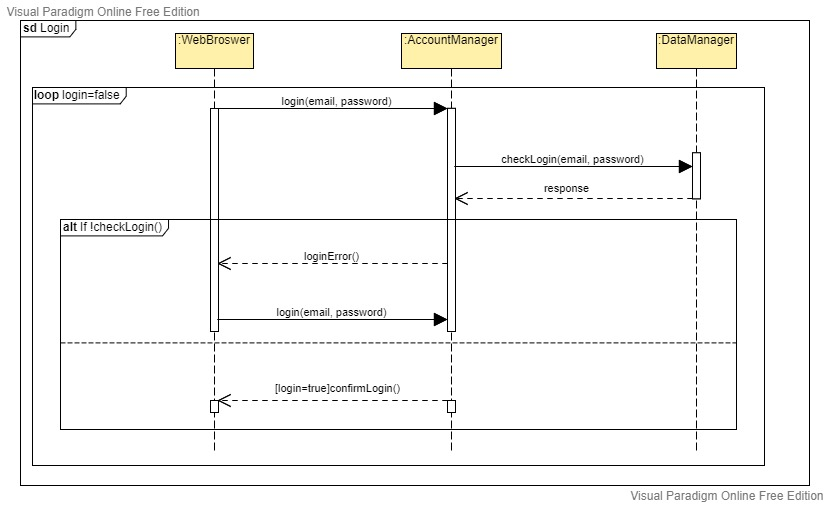
\includegraphics[scale=0.38, center]{assets/SequenceDiagram/SignUp.jpg}
        \caption{Sign Up phase}
        \label{fig:signup}
    \end{figure}
\end{center}
Sign up is the usual, user register itself by putting username, email, password job role and area. If the user is a farmer he put also the crop type.
Location module and Map service are used in this phase in order to allow the users to select their location using the GPS. 
However user can also choose to select manually its location without the use of GPS.

At the end of the process, if every checks were ok the user is saved into the database by the Data Manager component.

\newpage
\textbf{Log In}
\begin{center}
    \begin{figure}[H]
        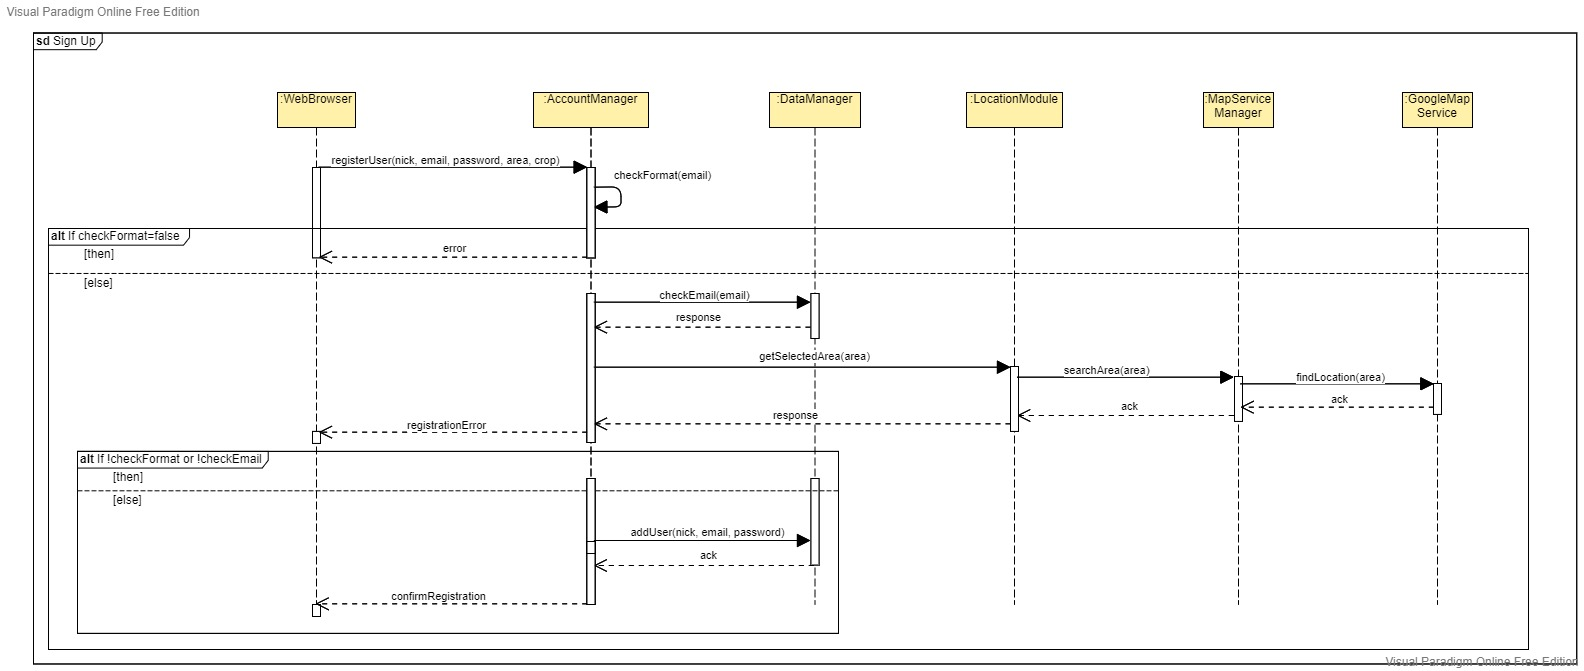
\includegraphics[scale=0.6, center]{assets/SequenceDiagram/Login.jpg}
        \caption{Login Phase}
        \label{fig: login}
    \end{figure}
\end{center}

Login phase is very simple, users put their email (primary and unique key of the database) and password and the sistem check if they're correct.
In case of success the user can log in the system and use its functionalities.
Every user will login the system accordingly the role that they had choosen in the Sign Up phase.

\newpage
\textbf{View Steering Initiative Reports}
\begin{center}
    \begin{figure}[H]
        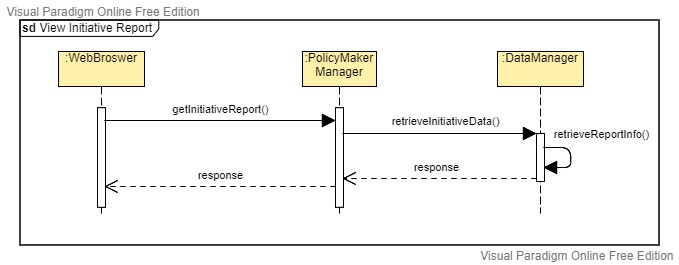
\includegraphics[scale=0.6, center]{assets/SequenceDiagram/Report.jpg}
        \caption{View Initiative reports}
        \label{fig: report}
    \end{figure}
\end{center}
This sequence diagram represents the interactions between components in order to display to the policy maker the steering initiative that are stored in the database.

\newpage
\textbf{Check Soil Humidity Data}
\begin{center}
    \begin{figure}[H]
        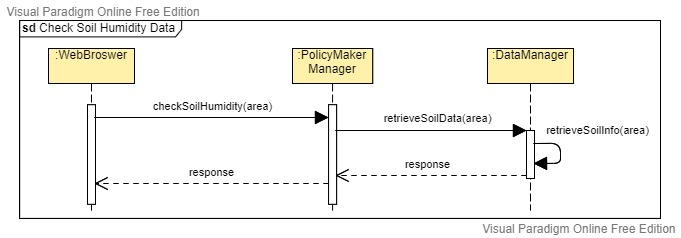
\includegraphics[scale=0.6, center]{assets/SequenceDiagram/Soil.jpg}
        \caption{Check Soil Humidity Sensors Data}
        \label{fig: humidity}
    \end{figure}
\end{center}
This sequence diagram represents the interactions between components in order to display to the policy maker the sensors data regarding the soil humidity.
These data are taken, by a """""""method"""""" in the application server, from an external source and they're put in the system database in order to manage them in a easiesr way.   

\newpage
\textbf{Check Water Irrigation Data} 
\begin{center}
    \begin{figure}[H]
        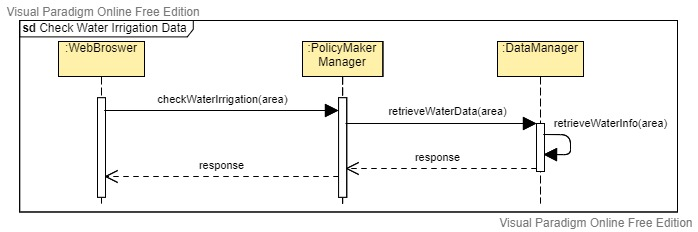
\includegraphics[scale=0.6, center]{assets/SequenceDiagram/Irrigation.jpg}
        \caption{Check Water Irrigation Sensors Data}
        \label{fig: irrigation}
    \end{figure}
\end{center}
This sequence diagram represents the interactions between components in order to display to the policy maker the sensors data regarding the water irrigation.
The function is the same that the case above.

\newpage
\textbf{View Farmers Ranking}
\begin{center}
    \begin{figure}[H]
        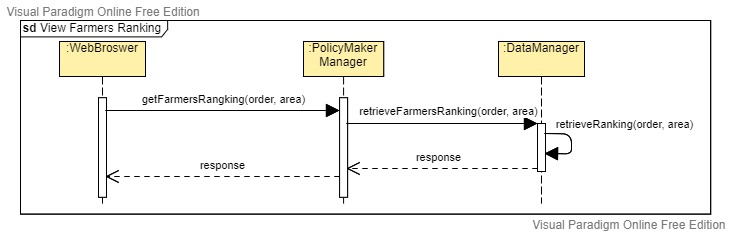
\includegraphics[scale=0.6, center]{assets/SequenceDiagram/Ranking.jpg}
        \caption{View Farmers Ranking}
        \label{fig: ranking}
    \end{figure}
\end{center}
This sequence diagram represents the interactions between components in order to display to policy makers and agronomists the ranking farmers ranking.
It will be explained better later in the document.
The function includes a parameter called 'area' in order to specify which area the user wants the rank.
In order to have code reusability this function can be used by either policy makers or agronomists. 
When a policy maker wants to see the rank the parameter 'area' will be set to 'all' in order to obtain the entire farmers rank.
Instead, when an agronomist wants to use it 'area' will be automatically taken from its responsibility area.  

\newpage
\textbf{View Specific Farmers Informations}
\begin{center}
    \begin{figure}[H]
        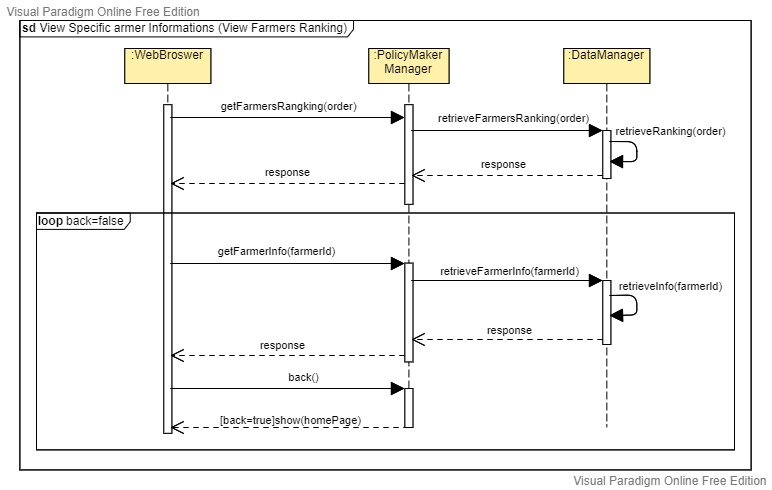
\includegraphics[scale=0.6, center]{assets/SequenceDiagram/SpecificFarmerInfo.jpg}
        \caption{View Specific Farmer Informations}
        \label{fig: specificFarmerInfo}
    \end{figure}
\end{center}
This sequence diagram represents the interactions between components to search for the informations of specific farmer information.

\newpage
\textbf{Profile Edit}
\begin{center}
    \begin{figure}[H]
        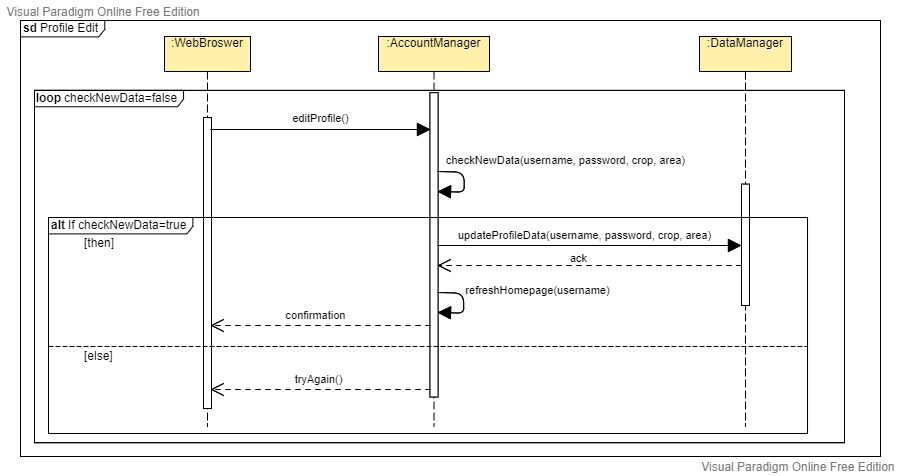
\includegraphics[scale=0.6, center]{assets/SequenceDiagram/ProfileEdit.jpg}
        \caption{Edit Profile}
        \label{fig: profileEdit}
    \end{figure}
\end{center}
This sequence diagram represents the interactions between components to change users profile settings like username, password, area or crop type if it's a farmer.

\newpage
\textbf{Insert Production Data}
\begin{center}
    \begin{figure}[H]
        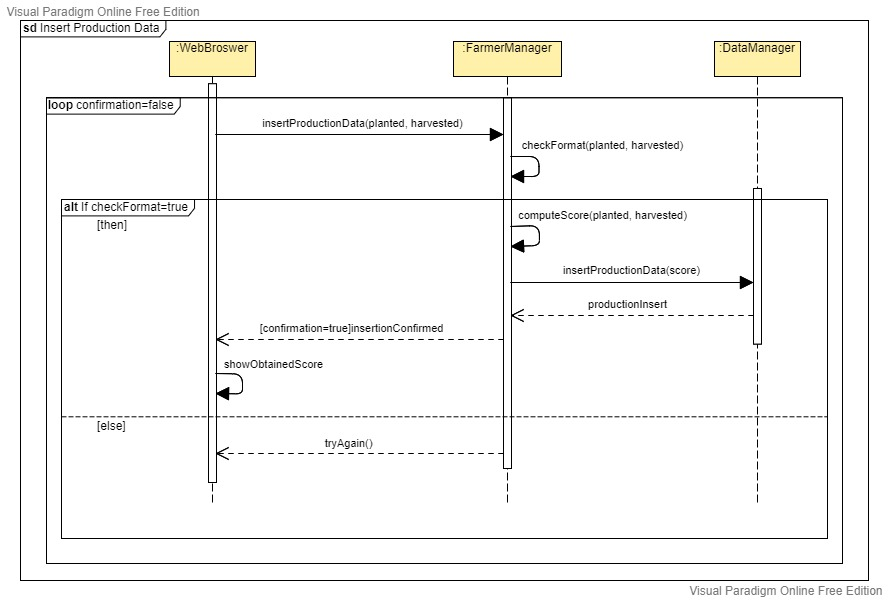
\includegraphics[scale=0.6, center]{assets/SequenceDiagram/InsertProduction.jpg}
        \caption{Insert Production Data}
        \label{fig: production}
    \end{figure}
\end{center}
This sequence diagram represents the interactions between components in order to insert farmers production data.
During this phase the rank is calculated in order to store it as an attribute of the farmer that insert the data.

\newpage
\textbf{Check News}
\begin{center}
    \begin{figure}[H]
        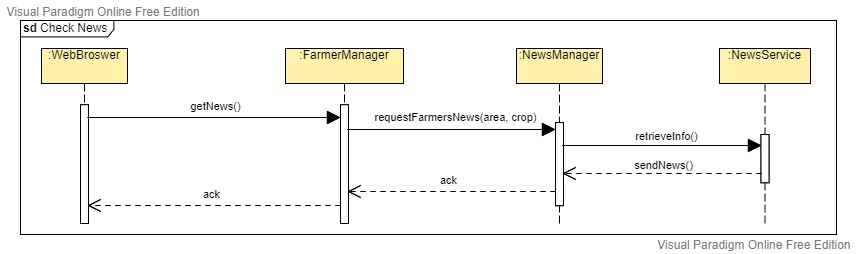
\includegraphics[scale=0.6, center]{assets/SequenceDiagram/CheckNews.jpg}
        \caption{Check News}
        \label{fig: news}
    \end{figure}
\end{center}
This sequence diagram represents the interactions between components in order to displays to the farmers the news regarding their interests, such as area or crop type.
It uses the NewsService component in order to get always up to date news and all it's managed by the NewsManager component.

\newpage
\textbf{Forum}
\begin{center}
    \begin{figure}[H]
        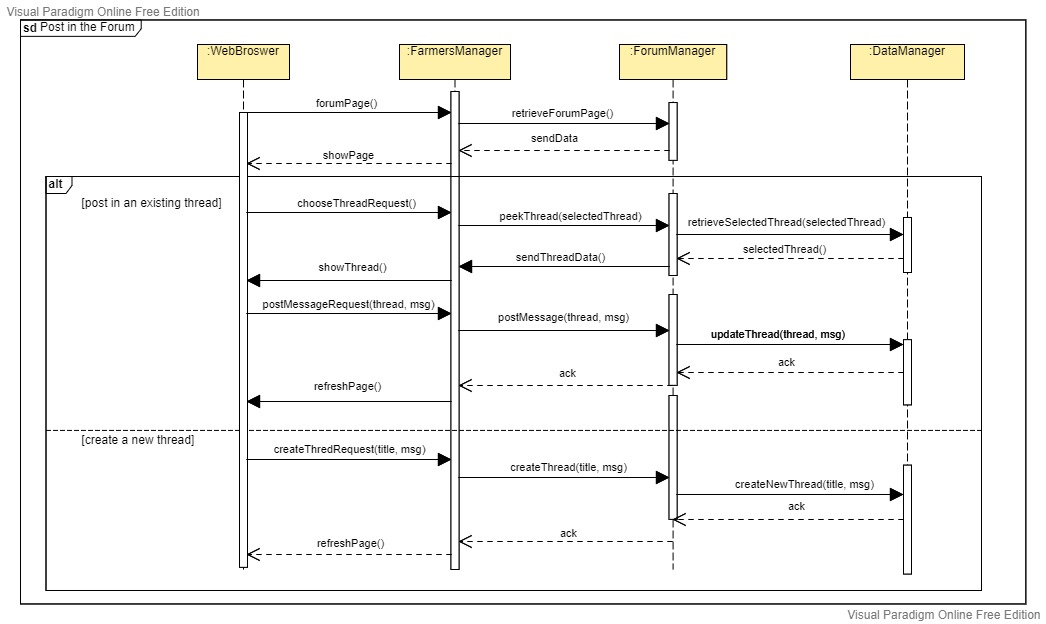
\includegraphics[scale=0.55, center]{assets/SequenceDiagram/Forum.jpg}
        \caption{Interact with Forum}
        \label{fig: forum}
    \end{figure}
\end{center}
This sequence diagram represents the interactions between the components composing the forum. 
It is split into two part the one that allows the user to make a post in an already existing thread and the one that allows the user to create a new thread.

\newpage
\textbf{Check Weathar Forecast}
\begin{center}
    \begin{figure}[H]
        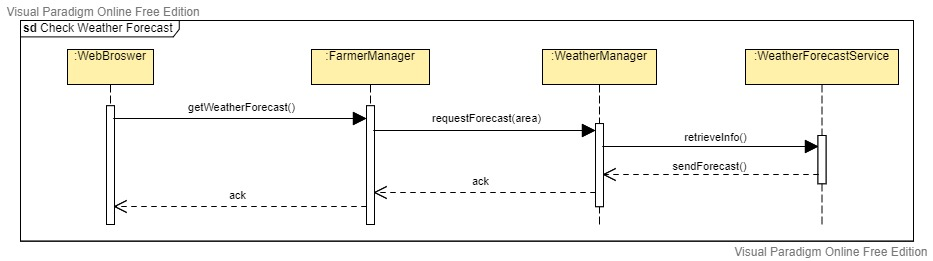
\includegraphics[scale=0.6, center]{assets/SequenceDiagram/Forecast.jpg}
        \caption{Check the Weather Forecasat}
        \label{fig: forecast}
    \end{figure}
\end{center}
This sequence diagram represents the interactions between components in order to displays to the users the weather forecast in relation to their area.
It uses the WeatherForecastService component in order to get always up to date forecast and all it's managed by the WeatherManager component.

\newpage
\textbf{Help Request Interaction}
\begin{center}
    \begin{figure}[H]
        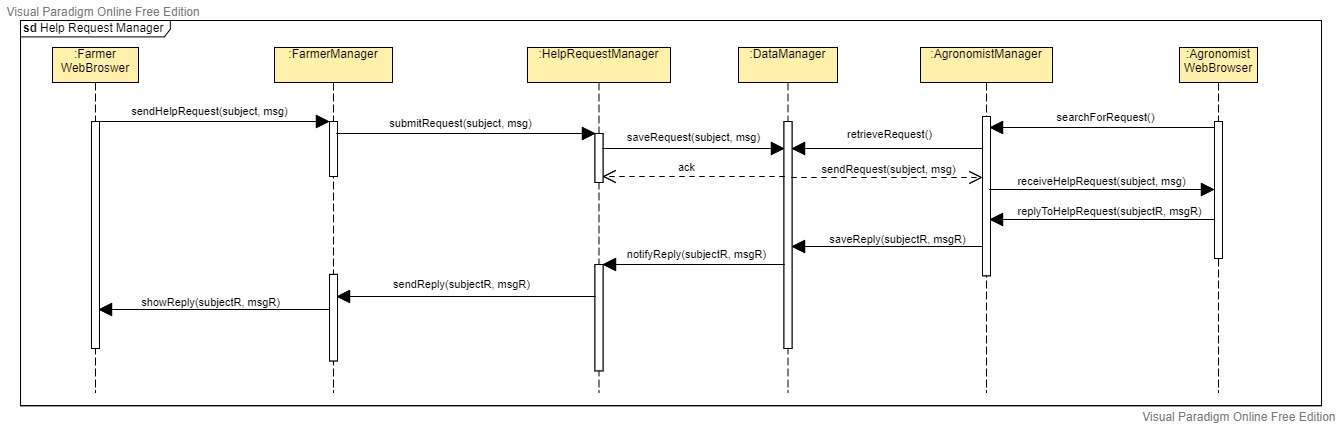
\includegraphics[scale=0.45, center]{assets/SequenceDiagram/HelpRequest.jpg}
        \caption{Help Request Interactions}
        \label{fig: helpRequest}
    \end{figure}
\end{center}
This sequence diagram represents the interactions between the components needed to manage the help request that the farmers send to the agronomists.
When a farmer send an help request the system save it in the database.
When the agronomist is online an automatic script checks if there are some unread messages in the database and sends them to the agronomist.
The agronomist replys to the request and saves it into the database. 
When the faremer is online another automatic script checks if there are some unread reply in the database and displays them to the farmer.
This method works also if one of the two actor is offline because the saving of the messages in the database.   

\newpage
\textbf{Daily Plan Management}
\begin{center}
    \begin{figure}[H]
        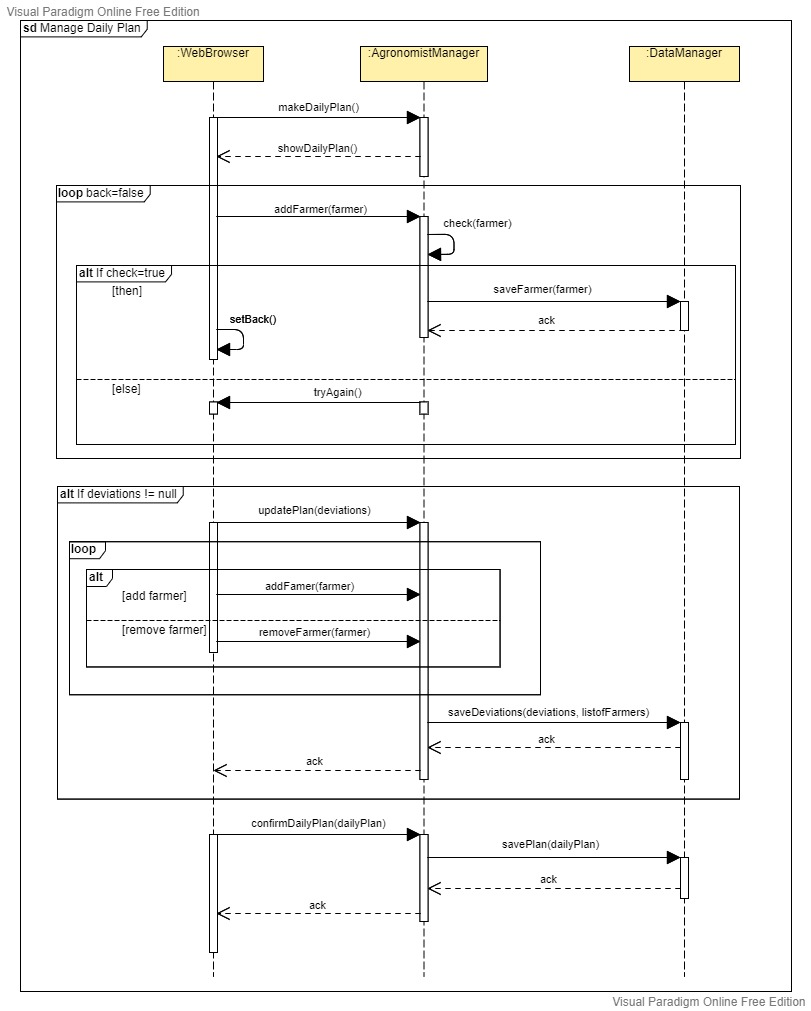
\includegraphics[scale=0.47, center]{assets/SequenceDiagram/DailyPlan.jpg}
        \caption{Daily Plan Interactions}
        \label{fig: dailyPlan}
    \end{figure}
\end{center}
This sequence diagram represents the interactions between components in order to manage the daily plan.
In the diagram are present either the creation and the updating of the plan.





\subsection{Component interfaces}

\subsection{Selected architectural styles and patterns}

\subsection{Other design decisions}

\section{User Interface Design}


\section{Requirements Traceability}


\section{Implementation, Integration and Test Plan}


\section{Effort Spent}


\section{References}


\end{document}